\documentclass{beamer}
\usepackage{graphicx,hyperref,udesc,url}
\usepackage[utf8]{inputenc}
\usepackage[T1]{fontenc}
\usepackage{booktabs}
\usepackage[portuges]{babel}

%%%%%%%%%%%%%%%%%%%%%%%%%%%%%%%%%%%%%%%%%%%%%%%%%%%%%%%%%%%%%%%%%%%%%

\title[Picat]{Picat: uma Linguagem Multiparadigma}

\author[Battisti \& PV]{
    João Herique Faes Battisti, Paulo Victor de Aguiar\\\medskip
    {\small \url{joaobattisti@gmail.com}} \\ 
{\small \url{pavaguiar@gmail.com}}}

\institute[UDESC]{
    Departamento de Ci\^encia da Computa\c{c}\~ao \\
    Centro de Ci\^encias e Tecnol\'ogias\\
Universidade do Estado de Santa Catarina}

%%%%%%%%%%%%%%%%%%%%%%%%%%%%%%%%%%%%%%%%%%%%%%%%%%%%%%%%%%%%%%%%%%%%%

\begin{document}

\begin{frame}
    \titlepage
\end{frame}

%%%%%%%%%%%%%%%%%%%%%%%%%%%%%%%%%%%%%%%%%%%%%%%%%%%%%%%%%%%%%%%%%%%%%

\begin{frame}[fragile]
\frametitle{Sumário}
\tableofcontents
\end{frame}

\section{Introdução}
\begin{frame}
    \frametitle{História}
    \begin{itemize}
      \item Foi criada em 2013 pelos cientistas da computação Neng-Fa Zhou e Jonathan Fruhman.
      \item Utilizou o B-Prolog como base de implementação, e ambas utilizam regras lógicas na programação.
      \item Picat 0.1 – Teve seu lançamento em Maio de 2013.
      \item Picat 1.0 – Foi lançada Abril de 2015.
      \item Sua atual versão é a 1.9 com lançamento em Maio de 2016
    \end{itemize}
\end{frame}

%%%%%%%%%%%%%%%%%%%%%%%%%%%%%%%%%%%%%%%%%%%%%%%%%%%%%%%%%%%%%%%%%%%%%

%\section{Isso é outra seção}
\begin{frame}
    \frametitle{Picat é Multiparadigma}
    \begin{itemize}
      \item Imperativo
      \item Funcional
      \item \underline{Lógico}
    \end{itemize}
\end{frame}

%%%%%%%%%%%%%%%%%%%%%%%%%%%%%%%%%%%%%%%%%%%%%%%%%%%%%%%%%%%%%%%%%%%%%

\begin{frame}
    \frametitle{Linguagem Multiparadigma}
    Motivo de existencia dos paradigmas?
    \begin{itemize}
      \item Velocidade de implementação
      \item Velocidade de execução
      \item Elegância do código
    \end{itemize}
\end{frame}

%%%%%%%%%%%%%%%%%%%%%%%%%%%%%%%%%%%%%%%%%%%%%%%%%%%%%%%%%%%%%%%%%%%%%

\begin{frame}
    \frametitle{Linguagem Picat}
    \begin{itemize}
      \item A terminologia de picat segue as bases teóricas da linguagem Prolog.
      \item Lógica de primeira-ordem onde objetos são chamados por Termos.
      \item O destaque de Picat é a sua natureza declarativa, funcional, tipagem dinâmica, sintaxe simples mas poderosas.
      \item PICAT é um anacronico onde cada letra representa uma característica marcante de sua funcionalidade.
    \end{itemize}
\end{frame}

%%%%%%%%%%%%%%%%%%%%%%%%%%%%%%%%%%%%%%%%%%%%%%%%%%%%%%%%%%%%%%%%%%%%%

\section{Características}
\begin{frame}
    \frametitle{Características: \textcolor{red}{P}-I-C-A-T}
    \textbf{Pattern-matching}:\\ 
    Utiliza o conceito de casamento padrão. 
    Um predicado define uma relação e pode ter zero ou várias respostas. 
    Uma função é um predicado especial que sempre retorna uma única resposta. 
    Ambos são definidos com regras de Picat, e seus predicados e funções seguem as regras do casamento.
\end{frame}

%%%%%%%%%%%%%%%%%%%%%%%%%%%%%%%%%%%%%%%%%%%%%%%%%%%%%%%%%%%%%%%%%%%%%

\begin{frame}
    \frametitle{Características: P-\textcolor{red}{I}-C-A-T}
    \textbf{Intuitive}:\\ 
    O Picat oferece atribuições e laços de repetições para a programação dos dias de hoje. 
    Uma variável atribuída pode imitar várias variáveis lógicas, alterado seu valor seguindo o estado da computação. 
    As atribuições são úteis para associar os termos, bem como utilizadas nas estruturas de laços repetitivos. 
\end{frame}

%%%%%%%%%%%%%%%%%%%%%%%%%%%%%%%%%%%%%%%%%%%%%%%%%%%%%%%%%%%%%%%%%%%%%

\begin{frame}
    \frametitle{Características: P-I-\textcolor{red}{C}-A-T}
    \textbf{Constraints}:\\ 
    Picat suporta a programação por restrições. 
    Dado um conjunto de variáveis, 
    cada uma possui um domínio de valores possíveis e restrições para limitar os valores a serem atribuídos nas variáveis. 
    O objetivo é atribuir os valores que satisfaçam todas as restrições. 
\end{frame}

%%%%%%%%%%%%%%%%%%%%%%%%%%%%%%%%%%%%%%%%%%%%%%%%%%%%%%%%%%%%%%%%%%%%%

\begin{frame}
    \frametitle{Características: P-I-C-\textcolor{red}{A}-T}
    \textbf{Actors}:\\ 
    Atores são chamadas orientadas à eventos.
		Em Picat, as regras de ação descrevem comportamentos dos atores.
		Um ator recebe um objeto e dispara uma ação. 
		Os eventos são postados via canais de mensagem e um ator pode ser conectado há um canal, verificar e/ou processar seus eventos postados no canal.
		Neste ponto, estes atores desempenham características de área de Inteligência Artificial, especificamente a áreas de planejamento e sistemas multi-agentes.   
\end{frame}

%%%%%%%%%%%%%%%%%%%%%%%%%%%%%%%%%%%%%%%%%%%%%%%%%%%%%%%%%%%%%%%%%%%%%

\begin{frame}
    \frametitle{Características: P-I-C-A-\textcolor{red}{T}}
    \textbf{Tabling}:\\ 
    Considerando que operações entre variáveis podem ser armazenadas parcialmente em uma tabela na memória, permitindo que um programa acesse valores já calculados.
		Assim, evita-se a repetição de operações já realizadas.
		Com esta técnica de memoization, o Picat oferece soluções imediatas para problemas de programação dinâmica.
\end{frame}

%%%%%%%%%%%%%%%%%%%%%%%%%%%%%%%%%%%%%%%%%%%%%%%%%%%%%%%%%%%%%%%%%%%%%

\begin{frame}
    \frametitle{Comparações}
    \begin{table}[!bh]
\centering
\caption{Comparativo entre algumas linguagens: \url{https://rosettacode.org/wiki/Language_Comparison_Table}}
\label{tabela_ling_refs}
{\tiny
%%%\begin{tabular}{c|c|c|c|c|c|c}\hline \hline
%\begin{tabular}{C{2cm}|C{1.4cm}|C{1.4cm}|C{1.4cm}|C{1.4cm}|C{1.4cm}|C{1.4cm}}\hline \hline
\begin{tabular}{p{2cm}|p{1cm}|p{1cm}|p{1cm}|p{1cm}|p{1cm}}\hline \hline
      &\textbf{C}  &  \textbf{Haskell} &  \textbf{Java} &  \textbf{Prolog} &  \textbf{P.I.C.A.T}\\ \hline \hline
	    
Paradigma(s)	                        & procedural                                    & funcional                               & orientado à objetos   &  lógico                                             & multi-paradigma \\
\hline 

Tipagem	        & fraca                                         & forte                                   & forte                  &  fraca                                                         & fraca \\
\hline 

Verificação de tipos	                & estático                                      & estático                                & estático                              & dinâmico                                   & dinâmico \\

\hline  
Possui segurança?	                & não                                             & sim                                      & sim                                            & não                                          & sim\\

\hline  
Possui coletor de lixo?	                        & não                                                                        & sim                 &  sim                  & sim                                     & sim \\

\hline  
Passagem de parâmetros	                &  valor & -                                       &  valor                                     &  valor & casamento \\

\hline   
Legibilidade	  & baixa   & média     & média &  média       & boa \\


\hline 
\hline
\end{tabular} 
}

\end{table}
\end{frame}

%%%%%%%%%%%%%%%%%%%%%%%%%%%%%%%%%%%%%%%%%%%%%%%%%%%%%%%%%%%%%%%%%%%%%

\begin{frame}
    \frametitle{Usos}
    A linguagem Picat pode ser utilizada para diversas funções:
    \begin{itemize}
     \item Acadêmica
     \item Industrial
     \item Pesquisas
    \end{itemize}
\end{frame}


%%%%%%%%%%%%%%%%%%%%%%%%%%%%%%%%%%%%%%%%%%%%%%%%%%%%%%%%%%%%%%%%%%%%%

\begin{frame}
    \frametitle{Sistema de Programação}
    \begin{itemize}
     \item Picat é uma linguagem de multiplataforma, disponível em qualquer arquitetura de processamento e também de sistema operacional
     \item Utiliza a extensão .pi em seus arquivos de código fonte. 
     \item Existem 2 modos de utilização do Picat: Modo linha de comando e Modo Interativo. 
    \end{itemize}
\end{frame}

%%%%%%%%%%%%%%%%%%%%%%%%%%%%%%%%%%%%%%%%%%%%%%%%%%%%%%%%%%%%%%%%%%%%%

\begin{frame}
    \frametitle{Vantagens}
    \begin{itemize}
     \item Enfatiza uma visão moderna e controlável em seu mecanismo de backtracking.
     \item Clareza em construir regras declarativas.
     \item Funções disponíveis numa sintaxe análoga a Haskell com um ambiente de programação análogo ao Python.
     \item Biblioteca é organizada em módulo a exemplo de Haskell e Python. 
    \end{itemize}
\end{frame}

%%%%%%%%%%%%%%%%%%%%%%%%%%%%%%%%%%%%%%%%%%%%%%%%%%%%%%%%%%%%%%%%%%%%%

\begin{frame}
    \frametitle{Desvantagens}
    \begin{itemize}
     \item Manteve as letras maiúsculas para variáveis, como feito no B-Prolog.
     \item A geração de um código executável ainda não é puro, ela ainda se encontra em desenvolvimento
     \item As estruturas de repetição, comparadas com outras imperativas, ficam com uma sintaxe diferente. 
    \end{itemize}
\end{frame}

%%%%%%%%%%%%%%%%%%%%%%%%%%%%%%%%%%%%%%%%%%%%%%%%%%%%%%%%%%%%%%%%%%%%%

\section{Tipos de Dados}
\begin{frame}
\frametitle{Tipos de Dados}
\begin{figure}[!ht]
\centering
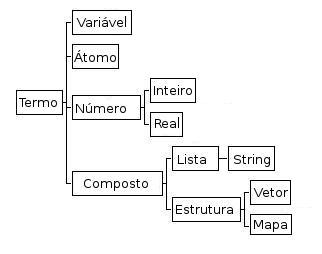
\includegraphics[width=.6\textwidth]{tipos_dados_picat_traduzido.jpg}
\caption{Hierarquia dos Tipos de dados}
\label{Hiera}
\end{figure}
\end{frame}

%%%%%%%%%%%%%%%%%%%%%%%%%%%%%%%%%%%%%%%%%%%%%%%%%%%%%%%%%%%%%%%%%%%%%

\begin{frame}
    \frametitle{Variável}
    \begin{itemize}
     \item As variáveis em Picat são similares as variáveis das matemática, pois ambas guardam valores. 
	   Diferentemente das linguagens imperativas, as variáveis em Picat não possuem um endereço simbólico na memória do computador.
     \item Quando uma variável ainda não foi instanciada com um valor, ela fica em um estado livre. 
	   Uma vez quando for instanciada com um valor, ela terá a mesma identidade como se fosse um valor até que ela seja liberada de novo.
    \end{itemize}
\end{frame}

%%%%%%%%%%%%%%%%%%%%%%%%%%%%%%%%%%%%%%%%%%%%%%%%%%%%%%%%%%%%%%%%%%%%%

\begin{frame}
    \frametitle{Átomo}
    \begin{itemize}
     \item Um átomo é uma constante simbólica e seu nome pode ser representado tanto com aspas simples ou sem. 
     \item Um átomo não pode ultrapassar uma linha de comando e seu nome tem um limite de mil caracteres. 
    
    Ex: x, x\_1, ’a’, ’b1’
    \end{itemize}
\end{frame}

%%%%%%%%%%%%%%%%%%%%%%%%%%%%%%%%%%%%%%%%%%%%%%%%%%%%%%%%%%%%%%%%%%%%%

\begin{frame}
    \frametitle{Número}
    \begin{itemize}
     \item Um número é um átomo inteiro ou real. Um número inteiro pode ser representado na forma decimal, binária, octal ou hexadecimal. 
     \item Já o número real usa o ponto no lugar da virgula para separar os valores depois de zero como: 3.1415.
    \end{itemize}
\end{frame}

%%%%%%%%%%%%%%%%%%%%%%%%%%%%%%%%%%%%%%%%%%%%%%%%%%%%%%%%%%%%%%%%%%%%%

\begin{frame}
    \frametitle{Número}
    \texttt{Picat> A = 5, B = 7, number(A), number(B),
    max(A, B) = Maximo, min(A, B) = Minimo.}\\
  
    \texttt{A = 5}\\
    \texttt{B = 7}\\
    \texttt{Maximo = 7}\\
    \texttt{Minimo = 5}\\
    \texttt{yes.}
\end{frame}

%%%%%%%%%%%%%%%%%%%%%%%%%%%%%%%%%%%%%%%%%%%%%%%%%%%%%%%%%%%%%%%%%%%%%

\begin{frame}
    \frametitle{Termos Compostos}
    Um termo composto se divide entre listas,  estruturas e outros tipos compostos derivado destes são: 
    \textit{strings}, vetores e mapas. Entretanto, ambos tem seus elementos acessados via casamento de padrões de fatos, predicados e funções.
\end{frame}

%%%%%%%%%%%%%%%%%%%%%%%%%%%%%%%%%%%%%%%%%%%%%%%%%%%%%%%%%%%%%%%%%%%%%

\begin{frame}
    \frametitle{Listas}
    A forma de uma lista reúne um conjunto de termos e os coloca dentro de colchetes: [t1; t2; :::; tn]. Veja o exemplo:
\end{frame}

%%%%%%%%%%%%%%%%%%%%%%%%%%%%%%%%%%%%%%%%%%%%%%%%%%%%%%%%%%%%%%%%%%%%%

\begin{frame}
    \frametitle{Listas}
    \texttt{Picat> A=[1,2,3], list(A), length(A)=L\_A, B= [4,5,6], list(B),}\\
    \texttt{length(B) = L\_B, A ++ B = C, list(C), length(C) = L\_C.}\\

    \texttt{A = [1,2,3]}\\
    \texttt{L\_A = 3}\\
    \texttt{B = [4,5,6]}\\
    \texttt{L\_B = 3}\\
    \texttt{C = [1,2,3,4,5,6]}\\
    \texttt{L\_C = 6}\\
    \texttt{yes.}
\end{frame}

%%%%%%%%%%%%%%%%%%%%%%%%%%%%%%%%%%%%%%%%%%%%%%%%%%%%%%%%%%%%%%%%%%%%%

\begin{frame}
    \frametitle{Estruturas}
    A forma de uma estrutura é definida como \$s(t1, t2, ..., tn),onde s é um átomo e \$ é usado para diferenciar uma função. 
    Seus principais elementos são o nome da estrutura que é o átomo que fica na frente e a aridade (número de argumentos do predicado). 
    Veja o exemplo:
\end{frame}

%%%%%%%%%%%%%%%%%%%%%%%%%%%%%%%%%%%%%%%%%%%%%%%%%%%%%%%%%%%%%%%%%%%%%

\begin{frame}
    \frametitle{Estruturas}
    \texttt{Picat> N = \$nome(1,2,3,4,5), struct(N), arity(N) = Aridade,}\\
    \texttt{to\_list(N) = Lista.}\\

    \texttt{N = nome(1,2,3,4,5)}\\
    \texttt{Aridade = 5}\\
    \texttt{Lista = [1,2,3,4,5]}\\
    \texttt{yes.}
\end{frame}

%%%%%%%%%%%%%%%%%%%%%%%%%%%%%%%%%%%%%%%%%%%%%%%%%%%%%%%%%%%%%%%%%%%%%

\begin{frame}
    \frametitle{Estruturas}
    \texttt{Picat> N = \$(1,2,3,4,5), struct(N), arity(N) = Aridade,}\\
    \texttt{to\_list(N) = Lista.}\\

    \texttt{N = (1,2,3,4,5)}\\
    \texttt{Aridade = 2}\\
    \texttt{Lista = [1,(2,3,4,5)]}\\
    \texttt{yes.}
\end{frame}

%%%%%%%%%%%%%%%%%%%%%%%%%%%%%%%%%%%%%%%%%%%%%%%%%%%%%%%%%%%%%%%%%%%%%

\section{Exemplos}
\begin{frame}
    \frametitle{Exemplos}
    \begin{figure}[!ht]
    \centering
    
\includegraphics[width=.6\textwidth]{exercicio.jpg}
    %\caption{Hierarquia dos Tipos de dados}
    %\label{Hiera}
    \end{figure}
\end{frame}

%%%%%%%%%%%%%%%%%%%%%%%%%%%%%%%%%%%%%%%%%%%%%%%%%%%%%%%%%%%%%%%%%%%%%

\begin{frame}
    \frametitle{Atribuição}
     \texttt{Picat> X := 7, X := X + 7, X := X + 7.}\\
     \texttt{X = 21}
\end{frame}

%%%%%%%%%%%%%%%%%%%%%%%%%%%%%%%%%%%%%%%%%%%%%%%%%%%%%%%%%%%%%%%%%%%%%

\begin{frame}
    \frametitle{Estruturas de Controle}
     \texttt{ex1 =>}\\
     \texttt{X:=3, Y:=4,}\\
     \texttt{if(X >= Y)}\\
     \texttt{then printf("\%d", X)}\\
     \texttt{else printf("\%d", Y)}\\
     \texttt{end.}
\end{frame}

%%%%%%%%%%%%%%%%%%%%%%%%%%%%%%%%%%%%%%%%%%%%%%%%%%%%%%%%%%%%%%%%%%%%%

\begin{frame}
    \frametitle{Soma até N}
    \texttt{Soma como predicado}\\
    \texttt{soma\_p(0,S) => S = 0.}\\
    \texttt{soma\_p(N,S), N > 0 =>}\\
    \texttt{\qquad \qquad \qquad \qquad \qquad soma\_p(N-1, Parcial),}\\
    \texttt{\qquad \qquad \qquad \qquad \qquad S = N + Parcial.}\\
		\texttt{}\\
		\texttt{Soma como Função - Classic}\\
		\texttt{soma\_f1(0) = S => S = 0.}\\
		\texttt{soma\_f1(N) = S, N >= 1 => S = N + soma\_f1 (N-1).}\\
		\texttt{}\\
		\texttt{Soma como função de fatos - próx. à Haskell}\\
		\texttt{soma\_f2(0) 0.}\\
		\texttt{soma\_f2(N) = N + soma\_f2 (N-1).}\\
\end{frame}

%%%%%%%%%%%%%%%%%%%%%%%%%%%%%%%%%%%%%%%%%%%%%%%%%%%%%%%%%%%%%%%%%%%%%

\begin{frame}
    \frametitle{Entradas e Saídas}
    \texttt{main =>}\\
    \texttt{printf("Digite dois números: "),}\\
    \texttt{N$\_real01 = read\_$real(),}\\
    \texttt{N$\_real02 = read\_$real(),}\\
    \texttt{Media = (N$\_real01+N\_real$02)/2,}\\
    \texttt{printf("A média é: \%6.2f", Media),}\\
    \texttt{printf("$\backslash n ......FIM....... \backslash$ n").}
\end{frame}

%%%%%%%%%%%%%%%%%%%%%%%%%%%%%%%%%%%%%%%%%%%%%%%%%%%%%%%%%%%%%%%%%%%%%

\section{Conclusão}
\begin{frame}
    \frametitle{Conclusão}
    \begin{itemize}
    \item PICAT é uma linguagem nova (2013), desconhecida, revolucionária e com um futuro promissor para áreas de pesquisas e utilização comercial.
    \item Atualmente há pouco material disponível e uma comunidade pequena de usuários, 
    mas existe um site atualizado e mantido por Hakan Kjellerstrand e um fórum de discussão no próprio site que está cada dia mais ativo, 
    graças ao crescimento de usuários desta linguagem.
    \end{itemize}
\end{frame}

%%%%%%%%%%%%%%%%%%%%%%%%%%%%%%%%%%%%%%%%%%%%%%%%%%%%%%%%%%%%%%%%%%%%%

%\section{Referências}
\begin{frame}
    \frametitle{Referências}
    \begin{itemize}
     \item \url{https://github.com/claudiosa/CCS/tree/master/picat}
     \item \url{http://picat-lang.org/}
    \end{itemize}
\end{frame}

%%%%%%%%%%%%%%%%%%%%%%%%%%%%%%%%%%%%%%%%%%%%%%%%%%%%%%%%%%%%%%%%%%%%%

%\section{Questionário}
\begin{frame}
    \frametitle{Questionário}
    \begin{enumerate}
     \item Qual característica do P.I.C.A.T é mais chamativa?
     \item Em quais aplicações você usaria P.I.C.A.T?
     \item Quais são os pontos positivos e negativos do P.I.C.A.T que você identifica?
     \item Se pudesse melhorar algo no P.I.C.A.T, o que melhoraria?
     \item O P.I.C.A.T pode substituir alguma linguagem?
    \end{enumerate}
\end{frame}

\end{document}
